\begin{figure}[H]
    \centering
    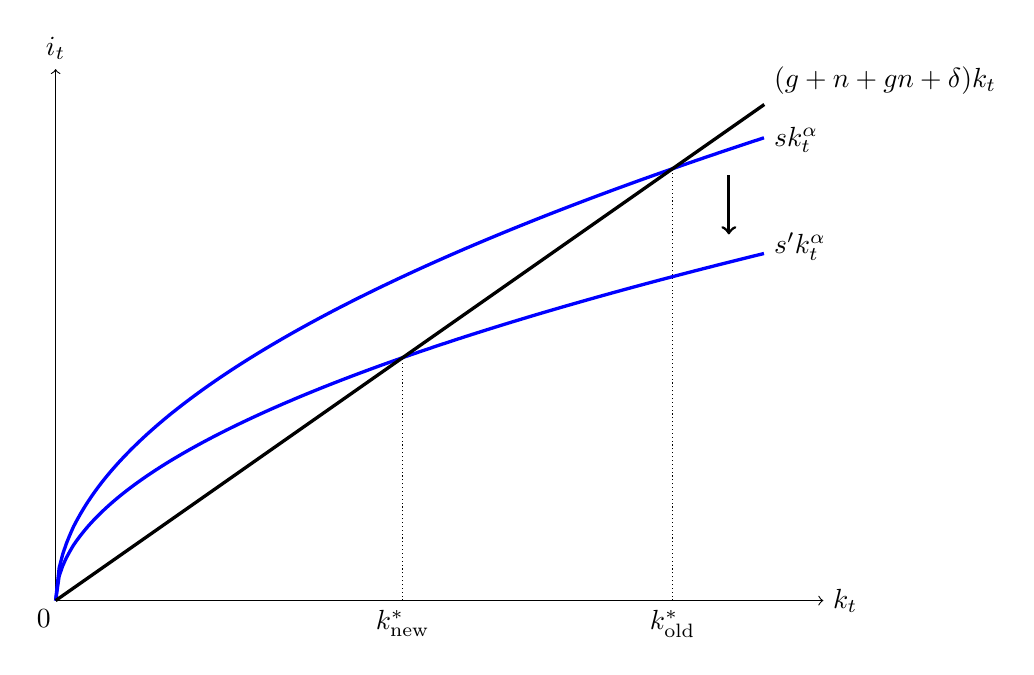
\begin{tikzpicture}[scale=1.5]
        \draw[->] (0, 0) -- (6.5, 0) node[right] {$k_t$};
        \draw[->] (0, 0) -- (0, 4.5) node[above] {$i_t$};
        \draw[densely dotted] (5.224,0) -- (5.224,3.657);
        \draw[densely dotted] (2.939,0) -- (2.939,2.057);
        \draw[domain=0:6, samples=200, blue, line width = 1.2pt, variable=\x] plot ({\x}, {1.6*(\x^0.5)});
        \draw[domain=0:6, samples=200, blue, line width = 1.2pt, variable=\x] plot ({\x}, {1.2*(\x^0.5)});
        \draw[domain=0:6, smooth, line width = 1.2pt, variable=\x] plot ({\x}, {0.7*\x)});
        \node at (-0.1,-0.15) {$0$};
        \node[right] at (6,4.4) {$(g + n + gn + \delta) k_t$};
        \node[right] at (6,3.9) {$s k_t^{\alpha}$};
        \node[right] at (6,3) {$s' k_t^{\alpha}$};
        \draw[->, line width=1pt] (5.7, 3.6) -- (5.7, 3.1);
        \node[below] at (2.939,0) {$k_{\rm new}^*$};
        \node[below] at (5.224,0) {$k_{\rm old}^*$};
    \end{tikzpicture}
\end{figure}